\chapter{软件设计}
这一章节主要介绍软件的开发过程,将软件按照功能逐步地进行细致划分,从而完成软件的设计任务。可能作为一个软件的使用者,认为软件很清楚地包括几个模块,几个功能,非常地清晰明了,自然很容易的实现。然而,这样的想法就如同觉得自己要是有一对翅膀就可以飞到月球一样幼稚。应该实现成什么样与怎样去实现它,二者之间有着巨大的沟壑。更何况,这两个中的每一个都可能有很多的设计方案,更不要说它们之间的组合了。
\section{软件框图}
如 \figurename{} \ref{fig:softarch} 为软件整体的关系图。
\begin{figure}[h]
	\centering
	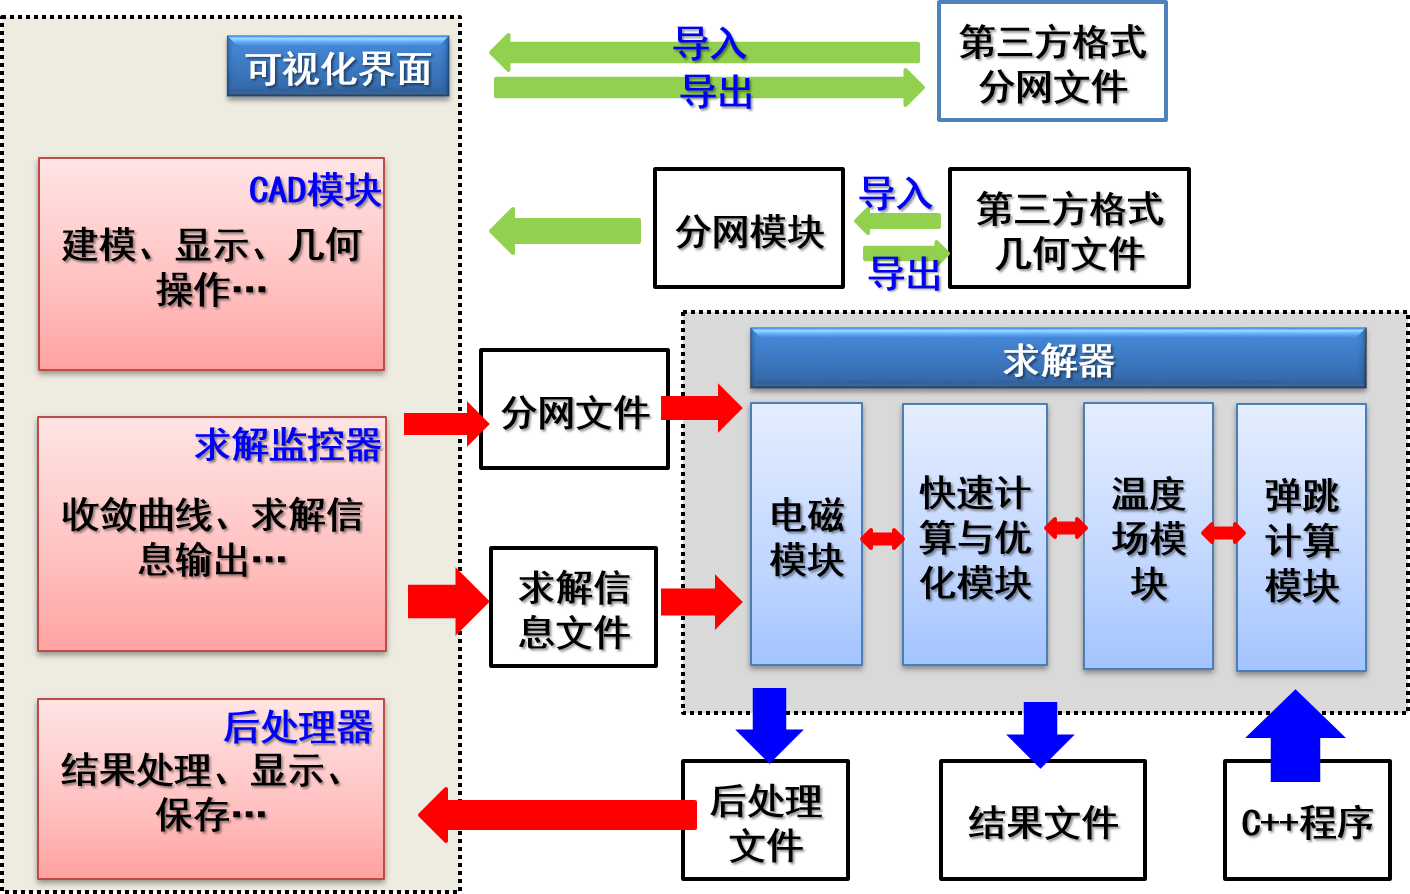
\includegraphics[width=0.7\linewidth]{figures/softarch}
	\caption{软件FEEM整体设计框架}
	\label{fig:softarch}
\end{figure}

\subsection{磁场问题的有限元求解}

\subsubsection{静磁场}

\subsubsection{瞬态磁场}
在电器当中的瞬态问题,主要还是考虑到可动部件的运动。

静态特性

在静态特性计算当中,可运动部件并没有真的在运动。只不过相对固定部分发生一定的位移之后,计算出电磁场的分布。求解的是一组静磁场问题。也没有考虑任何的动态方程,等同于针对位移的参数求解。

动态特性

实际的仿真过程需要考虑运动的耦合。电磁-运动的耦合是一种电磁问题和运动学问题的弱耦合。在每一个时间步的计算当中,先求解电磁场问题,然后再求解运动学问题,求解过程如下:

1.求解麦克斯韦方程组,计算发生一定位移后,施加在运动部件上的电磁力或电磁力矩;

2.求解运动部件的动态方程,计算出运动部件在时间步内的加速度值和速度,并且计算出下一时间步时运动部件新的位移位置;

3.将运动部件移动到新的位置,并且进行重分网操作;

4.返回步骤1。

\subsection{电磁力的计算}

Arkkio’s method


各种方法的优缺点对比

stress tensor方法的缺点

在数学上,这种方法是完全正确的,能够得到准确的力矩值,前提是B的计算值是准确的。然而,通常情况下不是这样的。需要注意的是,有限元求解是一种数值计算方法,因此,我们大多数情况下处理的都是近似值。特别地,我们实际求解得到的是磁势向量A,而磁感应强度B是通过计算A的旋度来得到的。这实际上是一个微分过程,如果我们对某些不准确的变量进行了微分操作,那么最后得到的计算结果必然也是有误差的。也就是说,我们计算得到的B的误差将会比A的误差更大。如果能够取消这个微分计算的过程,那么将有可能提高计算精度。
\subsection{优化问题}

\section{界面设计}

\subsection{Ribbon模块}
Ribbon模块是一个能够提供类似Office界面风格的组件。同时,COMSOL采用的也是类似界面。

1.如何自定义Ribbon的主题?
\subsection{QtFLEX模块}
该模块实现类似Visual studio当中的可停靠用户界面的组件。窗口内部的子部件可以根据用户随意的进行位置放置。可以设置自动隐藏停靠,可以与其他窗口进行分割,合并。
\begin{figure}
	\centering
	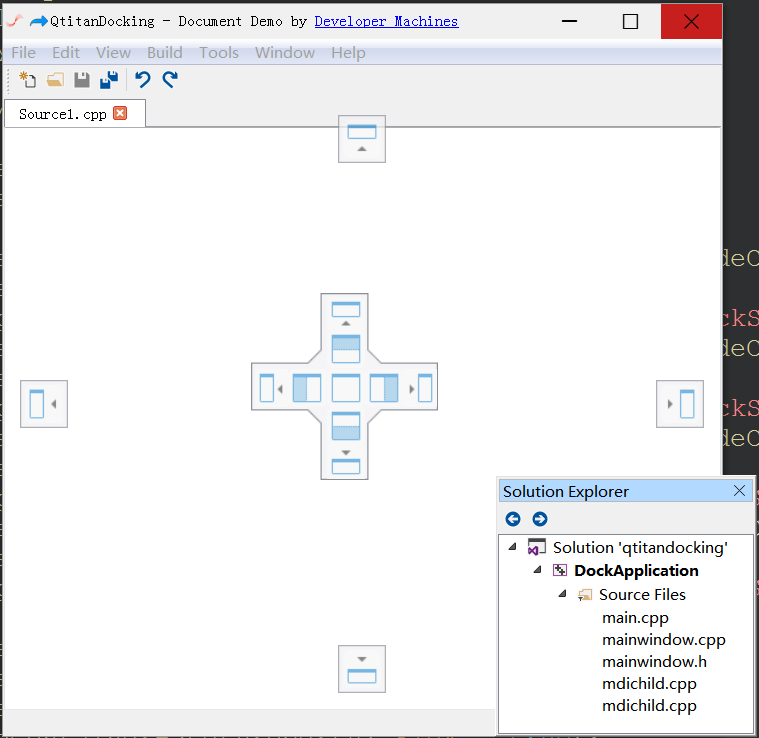
\includegraphics[width=0.7\linewidth]{figures/dock}
	\caption{Dock演示}
	\label{fig:dock}
\end{figure}

\subsection{界面布局}

\section{定义}
为了对数据进行存储,需要定义合理的格式和存储方式。
\subsection{工程文件格式及存储}
工程文件,即是软件会打开的文件,通过读取这个文件,软件可以获得该项目当中的几何模型、物理设置参数、分网信息、求解信息等。目前,最普遍的方式就是采用标记式语言进行存储,首选XML语言。
\subsection{几何文件格式及存储}
几何图形是用户在操作软件过程当中一直会使用到的东西,所以这部分数据肯定是常驻内存。在软件的核心,需要定义几何存储的格式来代表各种图形,这些图形可以是用户自己创建的,也可以是不同格式的几何文件转换过来的。
\subsection{分网文件格式及存储}
跟几何文件类似,也需要在工程内部自定义分网数据格式,来保存从各种格式的分网文件读取并转换而来的数据。
\subsection{结果数据文件及存储}
在求解结束后,需要一个数据结构来存储计算得到的各种数据结果。
\subsection{编程代码规范}
为了使软件开发尽量的规范,开发小组成员应当遵守以下操作:
\section{CAD绘图}
几何绘图是软件可视化最重要的一个部分。
\subsection{绘图原理}
在显示屏上你所看到的有趣的东西,都是程序员尽力地让一切看起来都跟真的似的,实际上,它依旧还是冷冰冰的机器,只是用的时间长了可能会发热而已。

\begin{enumerate}
	\item 图形的显示
	
\hspace*{2em} 图形在显示器上的显示效果,是我们通过程序进行渲染的结果。
	\item 图形的选中
	
\hspace*{2em} 图形的选中效果也是一种修饰,让用户感觉鼠标所单击的实体被选择了。实现方式就是绘制一个选中的效果,虚线框或者其他示意形状。那么如何方便的添加这个功能效果呢?简单的思路就是在每一个实体当作添加一个选中判断的函数,如果选中了,那么就返回一个相应的实体添加到选中实体的列表当中,然后调用重绘命令就可以了。
\end{enumerate}
\subsection{基本几何形状}
需要实现的基本几何形状有:点、线、圆弧、(长)方形、多边形、(椭)圆等。
\subsection{坐标网络的绘制}
绘制几何图形之前,需要建立一个绘制的画布,也就是具有横纵坐标的网格区域。需要注意的是,坐标轴上显示的数值跟屏幕上像素点的位置不是一样的,需要进行一下转化。

大多数的有限元仿真软件似乎不提供数学上的那种坐标轴网络,只有COMSOL是这样做的。我觉得提供一个坐标轴的显示还是比一个空白的背景要好很多。其实,flux2d也是有的,在你刚新建一个项目的时候会出现。
\begin{figure}
	\centering
	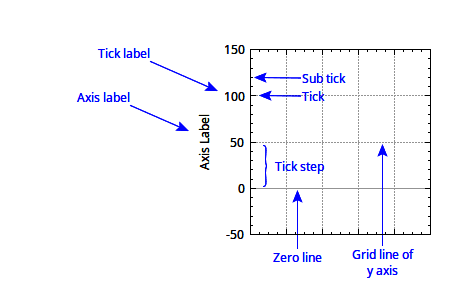
\includegraphics[width=0.7\linewidth]{figures/AxisNamesOverview}
	\caption{}
	\label{fig:axisnamesoverview}
\end{figure}
\begin{figure}
	\centering
	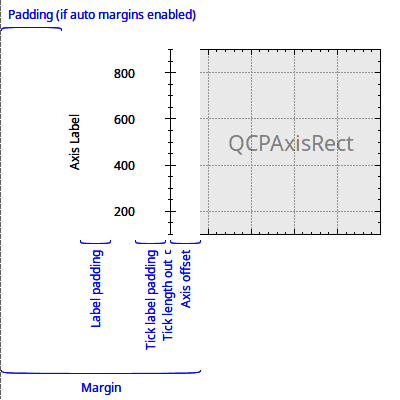
\includegraphics[width=0.7\linewidth]{figures/AxisRectSpacingOverview}
	\caption{}
	\label{fig:axisrectspacingoverview}
\end{figure}

接下来记录一下如何开发一个比较不错的简单坐标轴系统。

\begin{enumerate}
	\item 首先,需要建立一块画布,QWidget或者其子类,需要在上面进行绘图。这个画布类当中包含有各种画图需用的数据。
	\item 为了显示实际绘制的图形坐标而不是像素,需要一个基本的坐标轴,初始化的时候有一个默认的坐标轴大小区域。由于坐标轴的刻度与像素是一一对应的,所以,在绘制每一个图形之前,都需要调用坐标轴的转换函数来转换坐标,然后再绘制在画布上。需要注意的是,绘制的区域是有限制的,是被坐标轴所限制的,不能绘制在坐标轴之外。对于图形的缩放,似乎不需要特别处理,只需要更新一下坐标轴的范围,然后进行重画就可以了。
	\item 那么重头戏就是坐标轴了。
\end{enumerate}

主要功能:
\begin{enumerate}
	\item 状态栏显示鼠标指针所指的坐标轴内的坐标;
	\item 缩放功能;
	
\hspace*{2em} 可以在各种软件当作体验一下。以缩小为例,不断滚动鼠标滚轮,坐标轴网格会以鼠标指针所在的位置为中心缩小,缩小到一定程度子刻度网格不再显示,然后重新开始下一轮网格的缩放。坐标轴上的可以也会随缩放不断改变。
	\item 坐标轴外部不能绘图;

\hspace*{2em} 可以考虑clipRect函数。
\end{enumerate}

为了绘制一个长方形的坐标轴区域,在编程之前可以进行模块分解以及数据抽象。该长方形区域包含四个轴,因此可以抽象出“轴”这个类;然后对轴进行分解,可以包含轴线、刻度、刻度标签文本、网格等等,可以分别建立相应的类。
\subsection{形状操作}
所谓的用户能够对显示的几何形状进行控制,实际上是程序针对用户的鼠标操作与实际几何形状的位置进行了比较计算之后,进行了一些算法。每一次改变都会导致显示内容的刷新,只不过肉眼无法辨别出来。
\subsubsection{形状选中、调整大小、删除、隐藏显示}
每一个形状需要接受鼠标事件,单击可以被选中,绘制出被选中的效果,或者绘制外边框,或者改变形状的填充效果。

形状被选中后,可以进一步的调整形状的尺寸大小。外边框上会显示调控点。可以进一步地进行拖拽操作。

形状选中后,可以被移动到新的位置。
\subsubsection{自动吸附}
点坐标的自动捕捉,用来帮助我们快速地选择已有的一些点的坐标,方便进行图形的快速绘制。实现原理就是根据当前的鼠标坐标点,从几何实体列表当中去寻找,哪一个实体的哪一个点离该点最近,在捕捉精度范围内,那么该点就可以被捕捉到。如果是自由模式,就只捕捉当前的鼠标指针位置即可。
\subsubsection{布尔操作}

\subsubsection{缩放、变形}

\subsection{与分网显示、后处理的接口}

\subsection{参数绘图}

\section{材料库}
为了对模型当中的结构添加相应的材料属性,需要提供一个材料管理器的功能,能够存储一些常见的材料,并且能够实现新建、修改、删除等操作。
\subsection{已有材料库}

\subsection{新建、删除材料}

\subsection{导入、导出材料}

\section{分网生成}
分网无疑是有限元器求解最为关键的步骤之一。
\subsection{分网读取、导出}

\subsection{有限元分网形状}

\subsection{读取几何模型并分网}

\subsection{分网控制}

\subsection{删除分网}

\subsection{分网可视化}

\section{求解器}

\subsection{求解器设置}

\subsection{优化模块}
当所有的求解信息都设置好后,不仅可以实现磁场的求解,还能够实现对某些参数的优化设计。

\subsection{收敛曲线显示}

\section{后处理}
求解器计算得到的结果无疑要使用最好的方式展现给用户。
\subsection{结果曲线}

\subsection{结果云图}

\subsection{结果矢量图}

\subsection{数据导出}